\documentclass[conference]{IEEEtran}
\IEEEoverridecommandlockouts
\usepackage{cite}
\usepackage{amsmath,amssymb}
\usepackage{graphicx}
\usepackage{booktabs}
\usepackage{multirow}
\usepackage{adjustbox}
\usepackage{url}
\usepackage[hidelinks]{hyperref}
\graphicspath{{figures/}}

\begin{document}

\title{From Cloud Prompts to Local Models for Phishing Email Detection}

\author{
\IEEEauthorblockN{Arman Pyrbot\textsuperscript{*}, Anupam Udeniya, Kumar Saurabh}
\IEEEauthorblockA{\textit{School of Computer Science Engineering and Technology (SCSET)}\\
\textit{Bennett University}, Greater Noida, Uttar Pradesh, India\\
armanpyrbot@gmail.com, anupamudeniya2@gmail.com, pwc2017001@iiita.ac.in\\
\textsuperscript{*}Corresponding author}
}

\maketitle

\begin{abstract}
When a browser extension sends an email to a cloud-based large language model (LLM), the extension can check it for phishing. But this means that the email content is now shown to a third party for every checked email. And it comes with an API that is both required and paid. Also, typically, there is no quantitative analysis. We are therefore offering a Gmail extension, which replaces the cloud inference with locally trained models. The extension was developed and evaluated in three stages. Stage 1: we trained, quantized and stored a BERT model (BERT-tiny 4.4M) as a 4.48\,MB int8 ONNX graph that runs entirely in the browser. The median inference time is 5.2\,ms, and the test F1 is 0.9785 (0.9797 without quantization) on a group-disjoint split. Stage 2: we upgrade to BERT-small (28.8M). In-distribution F1 goes up to 0.9889. Inference time also grows to 125.8\,ms. For the out-of-distribution holdout of SpamAssassin, the false positive rate increases from 13.0\,\% to 15.7\,\%. Stage 3: we use a fine-tuned DeBERTa-v3-base model to get the score for the email text. An XGBoost classifier scores the links, and both models are served by a local Flask service. DeBERTa has an F1 of 0.9958 on a set of 20,926 held-out emails. The TF-IDF and logistic-regression baseline scores 0.9910. We deployed our fixed-weight fusion, which scores 0.9959. These results are in-distribution, because the split is not grouped by campaign and there is no external holdout. We also demonstrate that the classifier for the URL, which scores an F1 of 0.9980 for the page features on the test set of PhiUSIIL, classifies everything as phishing when given only the features that the service can calculate from the URL. When deployed, this adds an almost constant offset term and no real evidence.
\end{abstract}

\begin{IEEEkeywords}
phishing detection, browser extension, DeBERTa, XGBoost, late fusion, on-device inference, model quantization, large language models
\end{IEEEkeywords}

\section{Introduction}
Phishing is a common way for credentials to be stolen and for fraud to occur online. There were roughly 3.8 million phishing attacks recorded by the Anti-Phishing Working Group in 2025. The most active period was the second quarter, with 1,130,393 phishing attacks \cite{apwg2025q4}.

The arrival of large language models (LLMs) changes this situation. First, LLMs make it easier to create believable decoys \cite{heiding2024devising}. Second, they can parse incoming text and explain why it seems suspicious \cite{koide2024chatspamdetector}.

Pham \emph{et al.} \cite{pham2025demo} propose an extension for the browser which grabs the email message on the user's local machine.

It sends it to a Flask server which then ships it to the OpenAI GPT-4 API which returns a ``safe'', ``suspicious'' or ``phishing'' decision with a rationale.

It is a user-friendly tool but has three specific problems.

All the emails that are analyzed are shipped out of the user's machine.

It needs an API key, a constant connection and a pay-per-request plan.

There is no number associated with its accuracy and so it can't be benchmarked against other detectors.

We started off with a similar architecture (using Gemini to back a Flask endpoint), and slowly switched from remote inference to models that are trained, tested and hosted locally. This is the journey documented in this article. Here are our contributions:
\begin{itemize}
\item A staged migration away from a cloud LLM prototype with no accuracy measured to (i) an all-browser 4.4M params transformer, (ii) a bigger model with 28.8M params (all-browser), and (iii) a local service with a DeBERTa-v3 text classifier + XGBoost URL classifier. All three stages were quantitatively tested.\item A full-fledged Gmail Chrome Manifest V3 extension. It takes the subject, sender and body of the open message and sends them to a local service, which also extracts the embedded links. It responds with a risk classification, including probabilities per modality.\item A complete evaluation reporting accuracy, precision, recall, F1, ROC-AUC and confusion matrices, the effects of int8 quantization and in-browser latency, an out-of-distribution holdout for Stages 1 and 2, and a TF-IDF baseline with bootstrap confidence intervals for Stage 3.\item A discussion of what inflates or limits the reported numbers. It covers a document-format mismatch that made the first in-browser model fail silently on live Gmail pages, and a review of the deployed fusion rule and URL path, which shows that the URL branch's output saturates (stays near 1) on real email links.
\end{itemize}

\section{Related Works}
\subsection{Feature-based detection}
The original phishing email filters were based on hand-selected features. PILFER \cite{fette2007pilfer} focused on extracting script content, mismatched link text, and IP-based URLs as features and they found that random forests were the best performing classifier. Champa \emph{et al.} \cite{champa2024curated} consolidated a number of publicly available email data sets in a unified format and explored which attributes might be useful in separating phishing from legitimate emails. We use their compiled data set as the input to our final text model. For URLs, Prasad and Chandra's PhiUSIIL \cite{prasad2024phiusiil} contains 235,795 labeled URLs. These URLs contain features that are derived from lexical analysis and the page. We use these features for training our URL model.

\subsection{LLM-based detection}
Heiding \emph{et al.} \cite{heiding2024devising} demonstrate that GPT-4 can be used to create phishing emails. In their study, AI-written phishing emails reached click-through rates between 30 and 44\,\%. The AI-written messages performed better than the control group, but not as well as expert-created lures. Commercial LLMs can detect malicious intent as well, sometimes even better than humans. ChatSpamDetector \cite{koide2024chatspamdetector} can convert \texttt{.eml} files to prompts. Using GPT-4, it achieves 99.70\,\% accuracy and provides a natural language explanation for each decision. Thapa \emph{et al.} \cite{thapa2025quantized} analyze quantized open LLMs and classical detectors. Fine-tuned classic and deep models performed better than the quantized LLMs. The quantized LLMs were also heavy on GPU memory. Ganiuly and Smaiyl \cite{ganiuly2025trust} proposed a trustworthiness calibration framework. Their experiments show that, on average, GPT-4 was more trustworthy than LLaMA-3-8B and fine-tuned DeBERTa-v3-base. Sometimes reliability is not the same as accuracy.

\subsection{Fine-tuned transformers}
Fine-tuned models remain strong, low-cost baselines. For phishing email detection, Uddin and Sarker \cite{uddin2024explainable} applied fine-tuning to DistilBERT and presented an explanation for predictions via LIME and Transformer Interpret. SecureNet \cite{mahendru2024securenet} compared DeBERTa against LLMs and showed that DeBERTa has the highest recall (95.17\,\%), against GPT-4 (91.04\,\%). Al-Subaiey \emph{et al.} \cite{alsubaiey2024novel} developed an interpretable web platform for phishing email detection using a merged corpus that contains CEAS-08.

\subsection{Multimodal and webpage detection}
Lee \emph{et al.} \cite{lee2024mllm} applied multimodal LLMs to determine the brand imitated in the webpage and to check the domain. KnowPhish \cite{li2024knowphish} combined multimodal brand knowledge contained in the knowledge graph with an LLM. PhishAgent \cite{cao2025phishagent} extended the concept with an agent to look for information in online/offline knowledge. Altan \emph{et al.} \cite{altan2025dualpath} explored a DistilBERT text path and a classical URL classifier. They show the positive effect of combining the two. Our work is close to theirs.

\subsection{Client-side detection}
The closest approach to the first two stages of our work is PhishLang \cite{roy2026phishlang}. It runs MobileBERT on the actionable parts of a page's source code inside a Chromium extension, uses up to seven times less memory than comparable architectures, and flagged 25,796 phishing URLs during a 3.5-month deployment. Our browser stages work over the visible text of a message instead of the page source. We also show the impact of int8 quantization and the differences between browser and native runtime.

\section{Datasets}\label{sec:datasets}
\subsection{Unified Email and Webpage Corpus (Stages 1 and 2)}
The same corpus was used for the training of the in-browser models. This common corpus contains CEAS-08 (37,154 rows), and is based on a selection of emails across seven corpora (60,000), PhiUSIIL URL and pages (60,000), PhreshPhish (11,995) \cite{dalton2025phreshphish} with the addition of Nazario phishing corpus (1,565) and Nigerian fraud corpus (3,332). The SpamAssassin corpus (5,809 rows, 29.6\,\% phishing) was held out completely and never used for training. We pre-processed data by removing ASCII control characters, normalizing whitespaces, removing rows containing less than 12 characters, and eliminating 9,717 identical rows. For emails, we normalized rows to format of \texttt{[from]} sender \texttt{[body]} subject + body. For URLs, we used two fields: \texttt{[url]} and \texttt{[title]}.

\subsection{Curated Email Corpus (Stage 3)}
The final text model is trained on Champa \emph{et al.}'s curated email data \cite{champa2024curated}, the Spanish SpaPhish dataset \cite{spaphish2025} and a 909-message short-text set. After normalization, SHA-256 hashing and de-duplication, 139,502 messages were kept (73,347 phishing, 66,155 legitimate). The sources are listed in Table~\ref{tab:textdata}. We used a stratified 70/15/15 split, resulting in 97,651 training, 20,925 validation and 20,926 test messages. The test set contains 11,002 phishing messages and 9,924 legitimate messages. The test set contains 9,448 messages with at least one URL. SpamAssassin, the external holdout for Stages 1 and 2, is part of this corpus, so Stage 3 has no out-of-distribution test set.

\begin{table}[t]
\centering
\caption{Stage-3 text corpus after deduplication}
\label{tab:textdata}
\begin{tabular}{lrrr}
\toprule
Source & Legitimate & Phishing & Total \\
\midrule
TREC-07 & 23,747 & 29,392 & 53,139 \\
CEAS-08 & 17,294 & 21,841 & 39,135 \\
Enron & 15,474 & 13,950 & 29,424 \\
SpamAssassin & 4,091 & 1,716 & 5,807 \\
Nigerian fraud & 1,003 & 3,310 & 4,313 \\
Ling & 2,401 & 458 & 2,859 \\
Nazario & 961 & 1,560 & 2,521 \\
SpaPhish & 664 & 731 & 1,395 \\
Short text & 520 & 389 & 909 \\
\midrule
Total & 66,155 & 73,347 & 139,502 \\
\bottomrule
\end{tabular}
\end{table}

\subsection{PhiUSIIL URL Dataset (Stage 3)}\label{sec:url-data}
The URL model is trained on PhiUSIIL \cite{prasad2024phiusiil}. We reversed its labels, so 1 is phishing. Then we deleted duplicate rows on URL and label. This leaves 235,370 URLs (100,520 phishing URLs, 134,850 legitimate URLs). We have two kinds of splits. For the normal stratified split (70/10/20) we have 164,759 training URLs, 23,537 validation URLs, 47,074 test URLs. For the domain-aware split, \texttt{tldextract} extracts the registrable domain of every URL, and \texttt{StratifiedGroupKFold} is run twice over the whole dataset, grouped by that domain. This way, all URLs from one domain stay in the same split. The result is 188,296 training, 23,537 validation and 23,537 test URLs.

\section{Proposed Methodology}
This section gives a brief overview of the system architecture. It then describes pre-processing and feature engineering of data. The three detection pipelines are described with their training settings and run-time complexity. The assessment measures are presented at the end.

\subsection{System Architecture}
This overall architecture, as shown in Fig. \ref{fig:arch}, consists of three components: client-side extraction, two machine learning models and a decision engine.

\begin{figure*}[t]
\centering
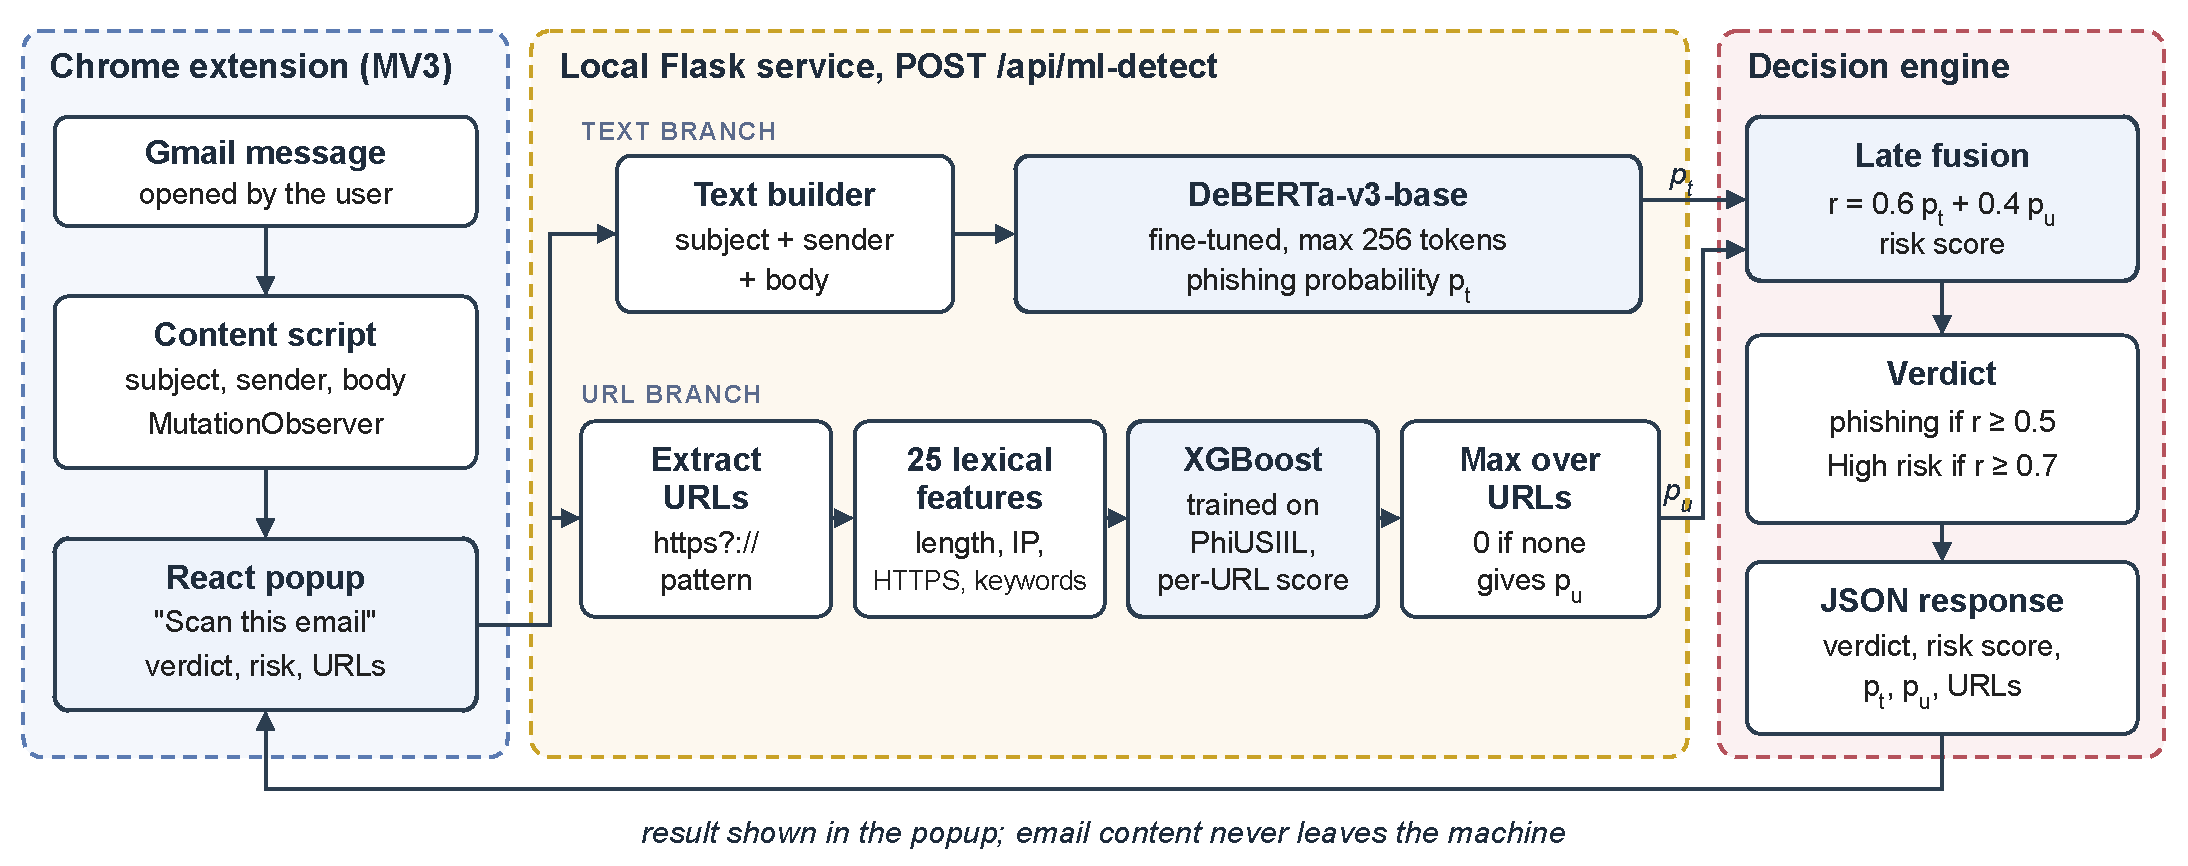
\includegraphics[width=\textwidth]{architecture.pdf}
\caption{High level architecture: Gmail extension extracts the open message. Local Flask server scores both text (DeBERTa-v3) and each URL (XGBoost). A decision engine takes both probabilities and calculates risk score which is displayed in popup.}
\label{fig:arch}
\end{figure*}

\textbf{Client-side extraction.} From Gmail's page, a content script will extract the subject (\texttt{h2.hP}), sender's email (\texttt{span.gD}), and message body (\texttt{div.a3s}). Gmail is a one-page UI so there is a debounced \texttt{MutationObserver} to make sure the data stays up to date as the page updates. The React popup (using React 19, built with Vite) will initially run \texttt{GET /api/health} and then send the message to \texttt{POST /api/ml-detect}, which is the Flask service running on a loopback address.

\subsection{Data Pre-processing}
We applied the cleaning/deduplication steps in Section \ref{sec:datasets} to each corpus. We then created the evaluation splits in such a way that it was never possible for a message/page that is a near-duplicate to be on both sides of the evaluation.

The aim is that no near-duplicates leak across splits. Thus, rows were grouped based on the registrable domain name (for rows representing URLs) or SHA-1 hash of sender + subject (for email rows, as a campaign proxy). Each of the groups was assigned to a single split (seed 42, 80/10/10). We have 123,479 training, 15,379 validation and 15,428 test rows, no common text, no common group across splits. Stage 2 used the same protocol. We added the 5,000 synthetic messages (Section \ref{sec:stage2}) before splitting the data. Thus the test set for Stage 2 (15,928 rows) is different to the test set for Stage 1. We have 546 synthetic rows in the test set for Stage 2 (277 BEC phishing and 269 legitimate). We have URL/page records (not email) for about 44\,\% of the test rows for both stages. Several source corpora (e.g. TREC, CEAS-08, SpamAssassin) were originally collected as spam corpora by their creators. For these sources, the positive class is a mix of phishing and other unsolicited emails. We take the labels as published. Counts per source differ from Stage 3 as different versions of corpora were used for different pipelines.

\subsection{Feature Engineering}
\textbf{Text model.} Subject + sender + body is concatenated, and truncated to 256 tokens. The string is then passed to a fine-tuned classifier (DeBERTa-v3-base) \cite{he2023debertav3}. And the text probability $p_t$ is the softmax probability value for the phishing class output from the classifier.

\textbf{URL model.} URLs are captured using the pattern \texttt{https?://[\textasciicircum\textbackslash s<>"]+}, and trailing punctuation is removed. Each URL is mapped to values for the 25 PhiUSIIL training features. These are length of URL, structure of domain, IP address hosts, obfuscation, character composition, HTTPS use, embedded redirect, social network domains, banking, payment and crypto keywords. An XGBoost classifier \cite{chen2016xgboost} then scores each URL. The highest score is used as the URL probability $p_u$ in the message (0 if no URLs). This maximization means that even one highly suspicious link will increase the URL signal.

\subsection{Proposed Detection Pipelines}
\subsubsection{Stage 1: in-browser BERT-tiny}
Our first local model is a fine-tuned \texttt{prajjwal1/bert-tiny} \cite{turc2019wellread} model, built from a two-layer BERT \cite{devlin2019bert} encoder with 128 hidden units and two attention heads, with a two-class linear head on top for a total of 4,386,178 parameters. After training, the model is exported to ONNX and dynamically quantized using ONNX Runtime \cite{onnxruntime} per the affine int8 strategy of Jacob \emph{et al.} \cite{jacob2018quantization}. This involves converting the MatMul weights to int8 and embedding tables to uint8 with per-tensor scaling. The weights and biases in LayerNorm remain float32. This reduces our artifact size from 17.6\,MB to 4.48\,MB.

The model ships as a Manifest V3 extension. It runs on a vendored ONNX Runtime Web 1.18, on a single WebAssembly thread \cite{onnxruntime}. Inference runs in the popup rather than in a service worker, because MV3 service workers stop when idle and the session would have to be rebuilt on every event. A handwritten WordPiece tokenizer (145 lines) matches the Hugging Face tokenizer on all 24 parity fixtures. The extension only requests the \texttt{activeTab} permission and makes no network calls during inference.

\subsubsection{Stage 2: in-browser BERT-small}\label{sec:stage2}
The second model switches the backbone to \texttt{prajjwal1/bert-small}, a four-layer encoder with 512 hidden units (28,764,674 parameters). We applied one label preserving augmentation (e.g. URL obfuscation, case/whitespace jitter) to every training row. This created 117,612 additional rows. Also we added 5,000 synthetic rows, a mix of polite business email compromise (BEC) phishing emails and ordinary business mail, before splitting. Total number of rows in train set became 245,073 (127,461 original + synthetic rows + 117,612 additional rows with augmentation). For 30\,\% of URL + title rows, we removed title, thus the model could also learn to work on URLs-only. At this stage we fixed an issue that the Stage-1 fixtures had missed: the old tokenizer did not separate Chinese, Japanese and Korean characters, so they collapsed into unknown tokens.

\subsubsection{Stage 3: fusion and decision engine}
\textbf{Decision engine.} The deployed service combines the two probabilities with fixed weights,
\begin{equation}
r = 0.6\,p_t + 0.4\,p_u ,
\label{eq:fusion}
\end{equation}
and ``phishing'' is declared when $r \ge 0.5$, ``high risk'' if $r \ge 0.7$, ``medium risk'' for any other phishing, and low risk in any other case.

The response carries the verdict, the risk level, the two component probabilities, the number of URLs, and the extracted URLs. If a model artifact is missing, HTTP 503 is returned and we don't resort to keyword rules. The weights and thresholds are fixed and hand-picked; we didn't use validation data to tune them.

A message without any links has $p_u = 0$. So it can't get higher than $r = 0.6$. We'll flag it as phishing only if $p_t \ge 0.833$ and it can't be ``high risk''.

We experimented with logistic-regression fusion as well, on $p_t$, $p_u$ and the URL count as an alternative to (\ref{eq:fusion}). We standardized the input and set balanced class weights.

\subsection{Training Configuration}
Table \ref{tab:hparams} is a summary of the training conditions for all the models. We trained the Stage 1 and Stage 2 models on an NVIDIA GeForce RTX 4060 Laptop GPU, taking 4.17 min and 43.12 min respectively. For getting base-size DeBERTa-v3 in a restricted GPU memory we used combination of mixed precision + gradient checkpointing + gradient accumulation and selected checkpoint that achieved the best validation F1. The XGBoost models used 500 trees, depth 8, learning rate 0.05, column and row subsampling of 0.8 (0.85 for the improved model), the \texttt{hist} tree method, and log-loss. The improved URL model adds 300 truncated-SVD components of a character 3--5-gram TF-IDF representation (sublinear term frequency, minimum document frequency of 3, at most 100,000 features), fitted on the training split only. Every split was generated with seed 42. As a classical baseline for the Stage 3 text model, we trained a TF-IDF and logistic-regression classifier on the same split (word 1--2-grams, minimum document frequency of 2, at most 200,000 features, sublinear term frequency, $C = 4$, untuned). F1 confidence intervals are from 1,000 bootstrap samples of test set. For the Stage 3 models we didn't track any hardware information or training time. And we didn't time the Stage 3 service.

\begin{table*}[t]
\centering
\caption{Configuration details for the training phase}
\label{tab:hparams}
\begin{tabular}{lccc}
\toprule
 & BERT-tiny & BERT-small & DeBERTa-v3 \\
\midrule
Model parameters & 4.39\,M & 28.76\,M & base (about 184\,M) \\
Maximum tokens & 192 & 256 & 256 \\
Optimizer & AdamW & AdamW & AdamW \\
Learning rate & $5\times10^{-5}$ & $3\times10^{-5}$ & $2\times10^{-5}$ \\
Effective batch size & 64 & 64 & 16 ($4\times4$) \\
Weight decay & 0.01 & not recorded & 0.01 \\
Learning-rate schedule & warmup 0.06 + cosine & cosine & linear, warmup 0.1 \\
Epochs (best) & 3 (3) & 5 (4) & 2 (2) \\
Early-stopping rule & val F1, patience 1 & patience 2 & none (best val-F1 checkpoint) \\
Additional settings & -- & label smoothing 0.05, AMP & AMP, grad. checkpointing \\
\bottomrule
\end{tabular}
\end{table*}

\subsection{Runtime Complexity}
Start with a transformer encoder that has $L$ layers and hidden size $d$. The number of operations needed to handle a token stream of length $n$ is roughly $L(n^2 d + n d^2)$ per message, limited by the largest input size: $n \le 192$ for BERT-tiny ($L = 2$, $d = 128$), and $n \le 256$ for BERT-small ($L = 4$, $d = 512$) and DeBERTa-v3-base ($L = 12$, $d = 768$). The number of operations needed for BERT-small is about 25$\times$ that of BERT-tiny, which is roughly the ratio between their median in-browser latencies (125.8\,ms vs.\ 5.2\,ms, see Table \ref{tab:ondevice}).

Using an XGBoost model with $T$ trees and depth $D$, scoring one URL after feature extraction requires up to $T D$ node comparisons ($T = 500$, $D = 8$). This feature extraction process has a cost proportional to URL length $|u|$. Then for one message containing $k$ links, there is an additional cost $O(k(|u| + T D))$. We used fusion rule (\ref{eq:fusion}), which requires constant time. We don't have a measurement for Stage-3 service latency. DeBERTa-v3-base, which has around 184M parameters, is expected to be the main cost for this stage.

\subsection{Evaluation Metrics}
TP, TN, FP and FN are the numbers of true positives, true negatives, false positives and false negatives for the phishing class. The metrics are:
\begin{equation}
\mathrm{Accuracy} = \frac{TP + TN}{TP + TN + FP + FN},
\label{eq:acc}
\end{equation}
\begin{equation}
\mathrm{Precision} = \frac{TP}{TP + FP}, \qquad \mathrm{Recall} = \frac{TP}{TP + FN},
\label{eq:pr}
\end{equation}
\begin{equation}
F_1 = \frac{2 \cdot \mathrm{Precision} \cdot \mathrm{Recall}}{\mathrm{Precision} + \mathrm{Recall}}, \qquad \mathrm{FPR} = \frac{FP}{FP + TN}.
\label{eq:prf}
\end{equation}

The receiver operating characteristic curve is a plot showing recall on the y-axis and FPR on the x-axis as the decision threshold is changed from 0 to 1. The area under it is the ROC-AUC.

We report accuracy, precision, recall, and F1 on the phishing class, plus a confusion matrix at the 0.5 threshold and threshold-free ROC-AUC.

For the in-browser models we report artifact size, time to load the model, median and 95th percentile of inference time (over 30 runs) in headless Chrome, the number of verdicts that change after int8 quantization, and the maximum probability difference between browser and native ONNX runtime on 24 fixtures.

\section{Results and Observations}


\subsection{Models running in the browser}
The in-browser models are compared in Table \ref{tab:ondevice}. BERT-small reduced the FP and FN on the in-distribution test set from 176 to 110 and from 161 to 78. After int8 quantization, 14 of 15,928 verdicts change for BERT-small (0.088\,\%), and 80 (0.52\,\%) for BERT-tiny. The maximum difference of int8 predictions between the browser and native runtime is reduced from 0.1626 to 0.0037. The performance on the SpamAssassin holdout is worse. On the holdout, BERT-tiny has a false-positive rate of 13.0\,\% and recall of 0.9051, while BERT-small has a false-positive rate of 15.7\,\% and recall of 0.9563. The ROC-AUC on the holdout drops from 0.9516 to 0.9209, so the transfer is worse for the larger model. Many emails in the legitimate class of SpamAssassin look like promotional emails that a phishing detector could reasonably flag. We didn't audit this, so the FP rates have this caveat. The numbers for the in-distribution test sets are also not directly comparable because the test sets are different. The Stage-2 test set includes 546 synthetic rows. The bigger size has a negative effect on the median inference time. It increases from 5.2\,ms to 125.8\,ms. That latency is still acceptable for a scan the user starts with a click.

\begin{table}[t]
\centering
\caption{In-browser models, evaluated at a 0.5 threshold}
\label{tab:ondevice}
\begin{adjustbox}{max width=\columnwidth}
\begin{tabular}{lcc}
\toprule
 & BERT-tiny & BERT-small \\
\midrule
Test rows & 15,428 & 15,928 \\
Accuracy (fp32) & 0.9782 & 0.9882 \\
Precision (fp32) & 0.9788 & 0.9871 \\
Recall (fp32) & 0.9806 & 0.9908 \\
F1 (fp32) & 0.9797 & 0.9890 \\
ROC-AUC (fp32) & 0.9975 & 0.9983 \\
False positives / false negatives (fp32) & 176 / 161 & 110 / 78 \\
False-positive rate (fp32) & 2.5\,\% & 1.5\,\% \\
F1 (int8, shipped) & 0.9785 & 0.9889 \\
int8 verdict changes & 80 (0.52\,\%) & 14 (0.088\,\%) \\
Model size fp32 / int8 & 17.6 / 4.48\,MB & 115.1 / 29.0\,MB \\
Load time & 301.1\,ms & 349.5\,ms \\
Inference median / p95 & 5.2 / 6.0\,ms & 125.8 / 138.3\,ms \\
Max browser-vs-native gap (int8) & 0.1626 & 0.0037 \\
\midrule
\multicolumn{3}{l}{\emph{SpamAssassin holdout, 5,809 rows, int8}} \\
Accuracy & 0.8804 & 0.8762 \\
Precision / Recall & 0.7451 / 0.9051 & 0.7184 / 0.9563 \\
F1 & 0.8173 & 0.8205 \\
ROC-AUC & 0.9516 & 0.9209 \\
False-positive rate & 13.0\,\% & 15.7\,\% \\
\bottomrule
\end{tabular}
\end{adjustbox}
\end{table}

\subsection{Case study: a document-format mismatch}
In the first Gmail test of the BERT-tiny extension, all four phishing emails were scored legitimate, each at about 0.003. We tried three extraction fixes: dropping an opaque webmail URL that used 104 of the 192 tokens, leaving out the sidebar text, and reading the message frame. None of them worked. Four different emails came back with almost the same score, so the model was scoring the Gmail interface and not the message. Scored directly, the four emails gave 0.83, 0.99, 0.99 and 1.00, but the document the extension put together gave between 0.01 and 0.13 even after those fixes. The input format was to blame. The training data had only two shapes, \texttt{[url]}+\texttt{[title]} for webpages and \texttt{[from]}+\texttt{[body]} for emails, while the extension was sending \texttt{[url]}+\texttt{[title]}+\texttt{[body]}. The model read that as a webpage and scored the mail client's own URL. We changed the extension to emit only shapes the model had seen, to drop the \texttt{[url]} line for known mail hosts and to read same-origin frames. After that, all four emails were caught, and a normal reply used as a control stayed legitimate. A polite invoice follow-up scored 0.5842: correct, but only 0.08 above the threshold. BERT-small, which was trained with synthetic BEC samples, gave the same email 0.9444.

\subsection{The final text model}
After its first epoch, DeBERTa-v3 had a validation F1 of 0.9912 (validation loss 0.0345), and after the second it was 0.9967 (validation loss 0.0153). On the test set of 20,926 messages, it achieved accuracy 0.9956, precision 0.9976, recall 0.9940, F1 0.9958 with 26 false positives, 66 false negatives, and an ROC-AUC of 0.9998 (Table \ref{tab:final}). The bootstrapped 95\,\% CI on its F1 is 0.9950--0.9966. The TF-IDF baseline achieved an F1 of 0.9910 (0.9897--0.9922). There were 114 false positives and 85 false negatives. The transformer is better, though only by about half a point. DeBERTa performed the worst on SpaPhish (F1 0.9536, false positive rate 6.4\,\%, $n = 227$) and SpamAssassin (F1 0.9658, $n = 885$). It performed the best on CEAS-08 (0.9986) and TREC-07 (0.9975).

\begin{table*}[t]
\centering
\caption{Final-stage held-out test set results (decision threshold 0.5). $^{\dagger}$Approximately 70\,\% of SpaPhish was in the training split for DeBERTa. Note that this row is not held out for the text model.}
\label{tab:final}
\begin{adjustbox}{max width=\textwidth}
\begin{tabular}{llrcccccc}
\toprule
Model & Test set & Test size ($n$) & Accuracy & Precision & Recall & F1 & ROC-AUC & TN / FP / FN / TP \\
\midrule
DeBERTa-v3 (text) & email, stratified & 20,926 & 0.9956 & 0.9976 & 0.9940 & 0.9958 & 0.9998 & 9,898 / 26 / 66 / 10,936 \\
TF-IDF + LR baseline & email, stratified & 20,926 & 0.9905 & 0.9897 & 0.9923 & 0.9910 & 0.9994 & 9,810 / 114 / 85 / 10,917 \\
Deployed rule (\ref{eq:fusion}) & email, stratified & 20,926 & 0.9957 & 0.9978 & 0.9940 & 0.9959 & 0.9971 & 9,900 / 24 / 66 / 10,936 \\
XGBoost, 25 PhiUSIIL features & PhiUSIIL, stratified & 47,074 & 0.9983 & 0.9983 & 0.9976 & 0.9980 & 0.99998 & 26,936 / 34 / 48 / 20,056 \\
XGBoost, 25 + 300 SVD & PhiUSIIL, domain-disjoint & 23,537 & 0.9978 & 0.9997 & 0.9951 & 0.9974 & 0.9989 & 13,482 / 3 / 49 / 10,003 \\
XGBoost, serving-time features & PhiUSIIL, stratified & 47,074 & 0.4271 & 0.4271 & 1.0000 & 0.5985 & 0.5240 & 0 / 26,970 / 0 / 20,104 \\
Learned fusion (not deployed) & email, stratified & 20,926 & 0.9957 & 0.9976 & 0.9941 & 0.9959 & 0.9989 & 9,898 / 26 / 65 / 10,937 \\
Learned fusion$^{\dagger}$ & SpaPhish subset & 210 & 0.9810 & 0.9818 & 0.9818 & 0.9818 & 0.9909 & 98 / 2 / 2 / 108 \\
\bottomrule
\end{tabular}
\end{adjustbox}
\end{table*}

\subsection{The URL model}
The 25-feature XGBoost model reached the F1 of 0.9980 and ROC-AUC 0.99998 on the 47,074 test URLs with respect to the feature values of the dataset. The gain based feature importance is rather dominated by the handful of features such as HasSocialNet (0.564), NoOfExternalRef (0.182), IsHTTPS (0.106) and NoOfOtherSpecialCharsInURL (0.071). Five features, IsDomainIP and the three obfuscation features among them, reached zero importance. Adding 300 SVD components of character n-grams and running on the domain-disjoint split brings the F1 to 0.9974 with only 3 false positives out of 13,485 legitimate URLs. These scores don't reflect the deployed path. The same 47,074 test URLs were rescored using the features derived from URL string that the service uses. All URLs were predicted as phishing (26,970 false positives). ROC-AUC is 0.5240. Legitimate pages of PhiUSIIL typically have social network links and external references. The service doesn't see them, thus it leaves them at zero or infers from the URL text. This is reflected in the actual emails too. On the test emails with at least one link, the mean $p_u$ for legitimate messages is 0.9988 and for phishing is 0.9995.

\subsection{Fusion}
The logistic regression fusion model, trained using DeBERTa/XGBoost predictions over 20,925 validation messages and tested on 20,926 test messages, achieves F1 0.9959 and ROC-AUC 0.9989, one more true positive than DeBERTa. The standardized coefficients are 11.219 for $p_t$, $-0.205$ for $p_u$, $-0.003$ for the URL count, with intercept $-5.166$, so on these corpora the decision rests almost entirely on the text. The other fusion model, trained on SpaPhish, gives positive weight to the URL probability (0.717 vs.\ 3.849 for $p_t$), and reaches F1 0.9818 over 210 test messages. On the full test set, the deployed rule (\ref{eq:fusion}) reaches F1 0.9959 with 24 false positives and 66 false negatives. Its bootstrap confidence interval is 0.9950--0.9967, overlapping DeBERTa's. They conflict on 20/20,926 emails. Since $p_u$ is almost always 1 for emails with any link, the rule in effect flags an email with a link once $p_t \ge 0.25$, and an email without a link once $p_t \ge 0.833$. Over the 11,478 messages with no URL, our recall (0.9925) is slightly worse than DeBERTa's at 0.5 (0.9937).

\subsection{Comparing the stages}
Table \ref{tab:stages} shows a summary. Notice that different corpora and different splits were used for every stage, so the rows cannot be compared directly; each row shows how a design did under its own protocol.

\begin{table}[t]
\centering
\caption{Stage-by-stage progression}
\label{tab:stages}
\begin{adjustbox}{max width=\columnwidth}
\begin{tabular}{lcccc}
\toprule
Stage & Deployment & Test size ($n$) & F1 (shipped) & Latency \\
\midrule
0: cloud LLM (our prototype) & remote API & -- & not recorded & network \\
1: BERT-tiny, int8 & in browser & 15,428 & 0.9785 & 5.2\,ms \\
2: BERT-small, int8 & in browser & 15,928 & 0.9889 & 125.8\,ms \\
3: DeBERTa-v3 alone & local service & 20,926 & 0.9958 & not measured \\
3: deployed rule (\ref{eq:fusion}) & local service & 20,926 & 0.9959 & not measured \\
\bottomrule
\end{tabular}
\end{adjustbox}
\end{table}

\subsection{Limitations and Threats to Validity}
These numbers are quite high, but there are a few caveats to consider here:

\emph{The URL branch does not work as deployed.} Given only the information that can be extracted from the link, the URL model flags every URL in the PhiUSIIL test set as phishing, and for links in actual emails it gives probabilities near 1 (regardless of the label). So the deployed rule is more or less just DeBERTa with two thresholds (0.25 for emails with links, 0.833 for emails without links). It has an F1 of 0.9959, which is almost the same as the one for DeBERTa alone. And the (not-deployed) learned fusion only differs from DeBERTa in a single test email and it gives a slightly negative weight to the URL probability. (Weights in Eq.~\ref{eq:fusion} are handpicked).

\emph{A training-to-serving gap.} Of 25 PhiUSIIL features, 9 describe the retrieved page (not the URL string). During inference, HasSocialNet, HasPasswordField, Bank, Pay, Crypto and NoOfURLRedirect are inferred from the URL text, while NoOfExternalRef, NoOfSelfRedirect and HasExternalFormSubmit are set to zero. NoOfExternalRef and HasSocialNet, the two most important training features, together account for 0.746 of the gain. During deployment these two features either get approximated or are missing. That's why we have a ROC-AUC of 0.5240 for the model. Also note the URL model was trained on the normal split (not domain disjoint) and on PhiUSIIL page labels (not links harvested from emails).

\emph{An optimistic SpaPhish fusion.} We trained/validated/tested the SpaPhish fusion on 976/209/210 of the 1,395 emails in SpaPhish. The 0.9818 F1 is optimistic, because about 70\,\% of those emails were also in DeBERTa's training split.

\emph{Split construction and external validity.} The Stage-3 text split (unlike Stages 1 and 2) only removes exact duplicates and does not group by campaign. Furthermore, there is no out-of-distribution holdout for Stage-3 (because SpamAssassin is in the training corpus), which means the headline numbers are in-distribution. The SpamAssassin numbers in Stages 1 and 2 (13.0\,\% and 15.7\,\% false-positive rates as opposed to 2.5\,\% and 1.5\,\% in-distribution) show how sharply performance can fall on previously unseen sources. All numbers come from a single training run (seed 42).

\emph{Scope and explanation.} The cloud LLM design \cite{pham2025demo} comes back with a rationale, but our local models return only a probability and a label. They see only the text and the URLs, not headers, attachments, images, certificates or redirects. The extension depends on Gmail's CSS selectors and sends the whole message over plain HTTP to the loopback service. That service has no authentication and accepts cross-origin requests from any origin. The probabilities are uncalibrated.

\section{Conclusion}
For a phishing-detection browser extension, we replaced the cloud LLM with locally trained models and evaluated each stage of the pipeline. An int8 BERT-tiny (4.48\,MB) in the browser can get F1=0.9785. It's offline, and requires 5.2\,ms per inference. The larger BERT-small pushes the in-distribution F1 to 0.9889 and catches a polite invoice-fraud email that the smaller model scored as borderline. But the out-of-distribution false-positive rate increases and the out-of-distribution ROC-AUC decreases. Finally, DeBERTa-v3 gets an F1=0.9958 on 20,926 emails. That is about half a point better than the TF-IDF baseline. Our deployed fusion rule practically matches it at 0.9959. But the URL classifier is the weak component. It does not transfer to serving features, and it just adds a nearly constant offset. Next, we will retrain the URL model on features that the link alone determines, and on links extracted from emails. We will introduce a campaign-grouped split, add an external holdout, measure the local service's latency, and calibrate the output probabilities. We will also bring back human-readable explanations with a small local generative model.

\bibliographystyle{IEEEtran}
\bibliography{refs}

\end{document}
